\documentclass[a4paper, 12pt]{article}

\def\languages{french, english}

%%%%%%%%%%%%%%%%%%% Libraries

%%%%%%%%%% Packages

\usepackage[
backend=biber,
style=numeric-comp,
sorting=none,
maxbibnames=99
]{biblatex}

%%%%%%%%%% Packages

%%%%% Coding tools

\usepackage{comment}
\usepackage{xstring}

%%%%% Encoding

\usepackage[utf8]{inputenc}
\usepackage[T1]{fontenc}
\usepackage{eurosym}

%%%%% Languages

\ifx\languages\undefined
	\usepackage[english]{babel}
\else
	\usepackage[\languages]{babel}
\fi

\def\languagefile{./include/languages/\languagename.tex}
\InputIfFileExists{\languagefile}{}

%%%%% Style

\usepackage{geometry}
\usepackage{fancyhdr}

\edef\restoreparindent{\parindent=\the\parindent\relax}
\usepackage[parfill]{parskip}

\usepackage{enumitem}
\usepackage{csquotes}
\usepackage{color}

%%%%% Others

\usepackage[framemethod=TikZ]{mdframed}
\usepackage[pdfusetitle]{hyperref}

%%%%%%%%%% Features

%%%%% Settings

\geometry{paper=a4paper,top=3.5cm,bottom=2.5cm,right=2.5cm,left=2.5cm}

\pagestyle{fancy}
\fancyhead[L]{}
\fancyhead[R]{\leftmark}
\fancyfoot[C]{\thepage}
\renewcommand{\headrulewidth}{0pt}

%\restoreparindent

%%%%% Commands

\newcommand{\romantableofcontents}{
	\newpage
	\pagenumbering{roman}
	\tableofcontents
	\newpage
	\pagenumbering{arabic}
}

%%%%%%%%%% Packages

\usepackage{float}
\usepackage[skip=1em]{caption}

\usepackage{array}
\usepackage{multirow}
\usepackage{multicol}

%%%%%%%%%% Features

%%%%% Settings

\renewcommand{\arraystretch}{1.2}

%%%%% Commands

\newcommand\noskipcaption[1]{\caption{#1}\vspace{-1em}}
\newcommand\noskipcaptionstar[1]{\caption*{#1}\vspace{-1em}}

%%%%%%%%%% Packages

\usepackage{inconsolata}
\usepackage{listings}

%%%%%%%%%% Features

%%%%% Commands

\newcommand{\Nstyle}[1]{
    \lstdefinestyle{N#1}{
        style=#1,
        %%%%%
        numbers=left
    }
}

\newcommand{\tbFstyle}[1]{
    \lstdefinestyle{tbF#1}{
        style=#1,
        %%%%%
        frame=tb
    }
}

\newcommand{\Fstyle}[1]{
    \lstdefinestyle{F#1}{
        style=#1,
        %%%%%
        frame=single,
        framesep=0em,
        rulesep=0em,
        xleftmargin=0.75em,
        xrightmargin=0.75em,
        framexleftmargin=0.75em,
        framexrightmargin=0.75em,
        framextopmargin=0.5em,
        framexbottommargin=0.5em,
        %%%%%
        numbersep=1.25em
    }
}

\newcommand{\NtbFstyle}[1]{
    \tbFstyle{#1}
    \Nstyle{tbF#1}
}

\newcommand{\NFstyle}[1]{
    \Fstyle{#1}
    \lstdefinestyle{NF#1}{
        style=f#1,
        %%%%%
        xleftmargin=2.75em,
        framexleftmargin=2.75em,
        %%%%%
        numbers=left,
        numbersep=1em
    }
}

%%%%% Styles

\lstdefinestyle{default}{
    breaklines=true,
    breakatwhitespace=true,
    columns=fixed,
	extendedchars=true,
    upquote=true,
	tabsize=4,
    %%%%%
    framerule=0.66pt,
    captionpos=b,
	%%%%%
    basicstyle=\footnotesize\ttfamily,
    numberstyle=\footnotesize\ttfamily,
    showstringspaces=false
}
\Nstyle{default}
\NFstyle{default}
\NtbFstyle{default}

\lstdefinestyle{monokai}{
    style=Fdefault,
    %%%%%
    backgroundcolor=\color[HTML]{272822},
    framerule=0em,
    %%%%%
    basicstyle=\footnotesize\ttfamily\color[HTML]{f8f8f2},
    numberstyle=\footnotesize\ttfamily\color[HTML]{272822},
    commentstyle=\color[HTML]{75715e},
    keywordstyle=[1]{\color[HTML]{f92672}},
    keywordstyle=[2]{\color[HTML]{A6E22E}},
    keywordstyle=[3]{\color[HTML]{ae81ff}},
    stringstyle=\color[HTML]{e6db74},
    %%%%%
    % otherkeywords={!,.,+,-,*,/,=,<,>,^,|,\&,OR,AND}
}

\lstdefinestyle{Nmonokai}{
    style=monokai,
    %%%%%
    xleftmargin=2.75em,
    framexleftmargin=2.75em,
    %%%%%
    numbers=left,
    numberstyle=\footnotesize\ttfamily\color[HTML]{f8f8f2},
    numbersep=1em
}

\lstdefinestyle{c}{
    language=C,
    style=default,
    %%%%%
    commentstyle=\color[HTML]{228B22},
    keywordstyle=\color[HTML]{0000FF},
    stringstyle=\color[HTML]{A020F0},
    emphstyle=\color[HTML]{0000FF},
    %%%%%
    emph={}
}

\lstdefinestyle{cpp}{
    language=C++,
    style=default,
    %%%%%
    commentstyle=\color[HTML]{228B22},
    keywordstyle=\color[HTML]{0000FF},
    stringstyle=\color[HTML]{A020F0},
    emphstyle=\color[HTML]{0000FF},
    %%%%%
    emph={std}
}

\lstdefinestyle{matlab}{
    language=matlab,
    style=default,
    %%%%%
    basicstyle=\footnotesize\fontfamily{pcr}\selectfont,
    numberstyle=\footnotesize\fontfamily{pcr}\selectfont,
    commentstyle=\color[HTML]{228B22},
    keywordstyle=\color[HTML]{0000FF},
    stringstyle=\color[HTML]{A020F0},
    emphstyle=\color[HTML]{0000FF},
    %%%%%
    emph={clearvars}
}

\lstdefinestyle{python}{
    language=python,
    style=default,
    %%%%%
    commentstyle=\color[RGB]{221,0,0},
    keywordstyle=[1]{\color[RGB]{255,119,0}},
    keywordstyle=[2]{\color[RGB]{144,0,144}},
    stringstyle=\color[RGB]{0,170,0},
    emphstyle=\color[RGB]{255,119,0},
    %%%%%
    emph={}
}

\lstdefinestyle{java}{
    language=java,
    style=default,
    %%%%%
    commentstyle=\color[HTML]{228B22},
    keywordstyle=\color[HTML]{0000FF},
    stringstyle=\color[HTML]{A020F0},
    emphstyle=\color[HTML]{0000FF},
    %%%%%
    emph={}
}

%%%%%%%%%% Packages

\usepackage{amsmath}
\usepackage{amssymb}
\usepackage{bm}
\usepackage{esint}
\usepackage[makeroom]{cancel}

%%%%%%%%%% Features

%%%%% Macros

\newcommand{\rbk}[1]{\left(#1\right)}
\newcommand{\cbk}[1]{\left\{#1\right\}}
\newcommand{\sbk}[1]{\left[#1\right]}
\newcommand{\abs}[1]{\left|#1\right|}
\newcommand{\norm}[1]{\left\|#1\right\|}

\newcommand{\fact}[1]{#1!}
\newcommand{\e}[1]{\mathbf{e}_{#1}}
\newcommand{\deriv}{\mathrm{d}}
\DeclareMathOperator{\tr}{tr}

\def\Rl{\mathbb{R}}
\def\Cx{\mathbb{C}}
\def\Na{\mathbb{N}}
\def\Zi{\mathbb{Z}}


%%%%% Settings

% lists
\frenchbsetup{StandardLists=true}

% units
\def\decimalsign{,}

% captions
\addto\captionsfrench{\def\figurename{Figure}}
\addto\captionsfrench{\def\tablename{Table}}
\addto\captionsfrench{\def\proofname{Preuve}}

% theorems

\def\lgthm{Théorème}
\def\lgprf{Preuve}
\def\lglem{Lemme}
\def\lgprop{Proposition}
\def\lgdefn{Définition}
\def\lghyp{Hypothèse}
\def\lgmeth{Méthode}
\def\lgquest{Question}
\def\lgansw{Réponse}
\def\lgexpl{Exemple}
\def\lgrmk{Remarque}
\def\lgnote{Note}
\def\lgtip{Conseil}

%%%%% Macros

\def\tq{\text{t.q.}}
\def\cad{c.-à-d.}
\def\Cad{C.-à-d.}


%%%%%%%%%% Packages

\usepackage{amsthm}
\usepackage{thmtools}

%%%%%%%%%% Features

%%%%% Settings

\makeatletter
\define@key{thmdef}{mdthm}[{}]{
	\thmt@trytwice{\def\thmt@theoremdefiner{\mdtheorem[#1]}}{}}
\makeatother

\begingroup
\makeatletter
\@for\theoremstyle:=plain,definition,remark\do{
	\expandafter\g@addto@macro\csname th@\theoremstyle\endcsname{
		\addtolength\thm@preskip\parskip
	}
}
\endgroup

\renewcommand{\qedsymbol}{$\blacksquare$}

% language

\ifx\lgthm\undefined
	\def\lgthm{Theorem}
	\def\lgprf{Proof}
	\def\lglem{Lemma}
	\def\lgprop{Proposition}
	\def\lgdefn{Definition}
	\def\lghyp{Hypothesis}
	\def\lgmeth{Method}
	\def\lgquest{Question}
	\def\lgansw{Answer}
	\def\lgexpl{Example}
	\def\lgrmk{Remark}
	\def\lgnote{Note}
	\def\lgtip{Tip}
\fi

%%%%% Commands

\newcommand\qedadd{\pushQED{\qed}\popQED}

%%%%% Environments

\theoremstyle{plain}
\newtheorem{thm}{\lgthm}
\newtheorem{lem}[thm]{\lglem}
\newtheorem{prop}[thm]{\lgprop}

\theoremstyle{definition}
\newtheorem{defn}{\lgdefn}
\newtheorem{hyp}{\lghyp}
\newtheorem{meth}{\lgmeth}
\newtheorem{quest}{\lgquest}

\theoremstyle{remark}
\newtheorem{answ}{\lgansw}[quest]
\newtheorem{expl}{\lgexpl}
\newtheorem*{rmk}{\lgrmk}
\newtheorem*{note}{\lgnote}
\newtheorem*{tip}{\lgtip}

% framed

\mdfdefinestyle{thicc}{
	nobreak=true,
	skipabove=\topskip,
	skipbelow=\topskip,
	innerleftmargin=0.5em,
	innerrightmargin=0.5em,
	innerbottommargin=0.5em,
	innertopmargin=0.5em,
	linewidth=0.25em,
	roundcorner=0.15em,
	linecolor=black!10,
	frametitlebackgroundcolor=black!10,
	theoremseparator={.}
}

\declaretheorem[mdthm={style=thicc, linecolor=red!20, frametitlebackgroundcolor=red!20}, sibling=thm, name=\lgthm]{framedthm}
\declaretheorem[mdthm={style=thicc, linecolor=red!20, frametitlebackgroundcolor=red!20}, sibling=thm, name=\lglem]{framedlem}
\declaretheorem[mdthm={style=thicc, linecolor=blue!20, frametitlebackgroundcolor=blue!20}, sibling=thm, name=\lgprop]{framedprop}
\declaretheorem[mdthm={style=thicc, nobreak=false}, parent=thm, name=\lgprf]{framedprf}

\declaretheorem[mdthm={style=thicc, linecolor=black!20!green!20, frametitlebackgroundcolor=black!20!green!20}, sibling=defn, name=\lgdefn]{frameddefn}
\declaretheorem[mdthm={style=thicc, linecolor=blue!20, frametitlebackgroundcolor=blue!20}, sibling=hyp, name=\lghyp]{framedhyp}
\declaretheorem[mdthm={style=thicc}, name=\lgmeth]{framedmeth}
\declaretheorem[mdthm={style=thicc, linecolor=orange!20, frametitlebackgroundcolor=orange!20}, sibling=quest, name=\lgquest]{framedquest}

\declaretheorem[mdthm={style=thicc, nobreak=false}, sibling=answ, name=\lgansw]{framedansw}
\declaretheorem[mdthm={style=thicc, nobreak=false}, sibling=expl, name=\lgexpl]{framedexpl}

%%%%%%%%%% Packages

\usepackage{siunitx}

%%%%%%%%%% Features

%%%%% Settings

\ifx\decimalsign\undefined
\else
    \sisetup{output-decimal-marker = \decimalsign}
\fi


%%%%%%%%%%%%%%%%%%% Titlepage

\def\logopath{/Users/maximemeurisse/Documents/LaTeX/personal/resources/pdf/logo-uliege.pdf}
\def\toptitle{University of Liège}
\title{Project (part 1) : Battleship}
\def\subtitle{Introduction to computer networking}
%\def\authorhead{AUTHOR}
\author{Maxime \textsc{Meurisse} (20161278)\\}
%\def\rightauthorhead{}
%\def\rightauthor{}
\def\context{3\ieme{} year of Bachelor Civil Engineer}
\date{Academic year 2018-2019}

%%%%%%%%%%%%%%%%%%%

\fancyhead[R]{}

%%%%%%%%%%%%%%%%%%% Document

\begin{document}
	%%%%%%%%%% Packages

%%%%% Coding tools

\usepackage{comment}
\usepackage{xstring}

%%%%% Encoding

\usepackage[utf8]{inputenc}
\usepackage[T1]{fontenc}
\usepackage{eurosym}

%%%%% Languages

\ifx\languages\undefined
	\usepackage[english]{babel}
\else
	\usepackage[\languages]{babel}
\fi

\def\languagefile{./include/languages/\languagename.tex}
\InputIfFileExists{\languagefile}{}

%%%%% Style

\usepackage{geometry}
\usepackage{fancyhdr}

\edef\restoreparindent{\parindent=\the\parindent\relax}
\usepackage[parfill]{parskip}

\usepackage{enumitem}
\usepackage{csquotes}
\usepackage{color}

%%%%% Others

\usepackage[framemethod=TikZ]{mdframed}
\usepackage[pdfusetitle]{hyperref}

%%%%%%%%%% Features

%%%%% Settings

\geometry{paper=a4paper,top=3.5cm,bottom=2.5cm,right=2.5cm,left=2.5cm}

\pagestyle{fancy}
\fancyhead[L]{}
\fancyhead[R]{\leftmark}
\fancyfoot[C]{\thepage}
\renewcommand{\headrulewidth}{0pt}

%\restoreparindent

%%%%% Commands

\newcommand{\romantableofcontents}{
	\newpage
	\pagenumbering{roman}
	\tableofcontents
	\newpage
	\pagenumbering{arabic}
}

	\section{Software architecture}
	The problem was to make a simplified version of the {\it Battleship} game between a client and a server using Java sockets.\par
	In order to solve this problem, I took advantage of the Java object-oriented paradigm and created several classes:
	\begin{itemize}
		\item \texttt{BattleshipClient} : this class implemented the client side of the game;
		\item \texttt{BattleshipServer} : this class implemented the server side of the game;
		\item \texttt{Entity} : this class represents an element of the game grid (a ship or an empty slot);
		\item \texttt{GameManager} : this class takes care of starting a game and managing it (shooting a position and displaying the status of the game);
		\item \texttt{Grid} : this class implements the game grid;
		\item \texttt{ServerWorker} : this class deals with managing the game of a player on the server side.
	\end{itemize}
	The details of each class and their methods are clearly explained in the code. In the remainder of this report, only the major points that helped manage the requests will be discussed.
	\subsection{\texttt{BattleshipClient}}
	This class interacts directly with the client via the terminal.\par
	First, it sends a request for a new game on port \texttt{2278}. When it receives the response from the server, if it is positive ({\it i.e.} if the server did not reject the connection), a menu with several choices is presented to the user:
	\begin{enumerate}
		\item {\bf Try a tile} : the client chooses a position in the grid to attack. This one, if it is valid, is sent to the server via a request (\texttt{1 1 position}). When the server response has been received, a message indicating which ship has been hit is displayed;
		\item {\bf See game status} : the client sends a request (\texttt{1 2}) to the server to obtain the list of the positions he has already attacked and the ship touched (or not) at each position. When the server response is received, each position-ship (or not) pair is displayed;
		\item {\bf Quit} : End the game (but does not stop the server thread).
	\end{enumerate}
	\subsection{\texttt{BattleshipServer}}
	The server listens on port \texttt{2278}. With each new connection received, it starts a new game on a new thread.
	\subsection{\texttt{GameManager}}
	This class implements the game itself. It creates a new grid and initializing it. It has methods to attack a position, display the status of the game and get the list of positions already attacked.\par
	When the server starts a new game on a new thread, this class is instantiated.
	\subsection{\texttt{Grid}}
	This class represents a game grid. The grid is a one-dimensional array with 100 elements (because in this case, the size of the grid is 10x10). As stated in the client, the coordinates of the grid are represented as shown in figure \ref{fig:grid}.\par
	\begin{figure}[!ht]
		\centering
		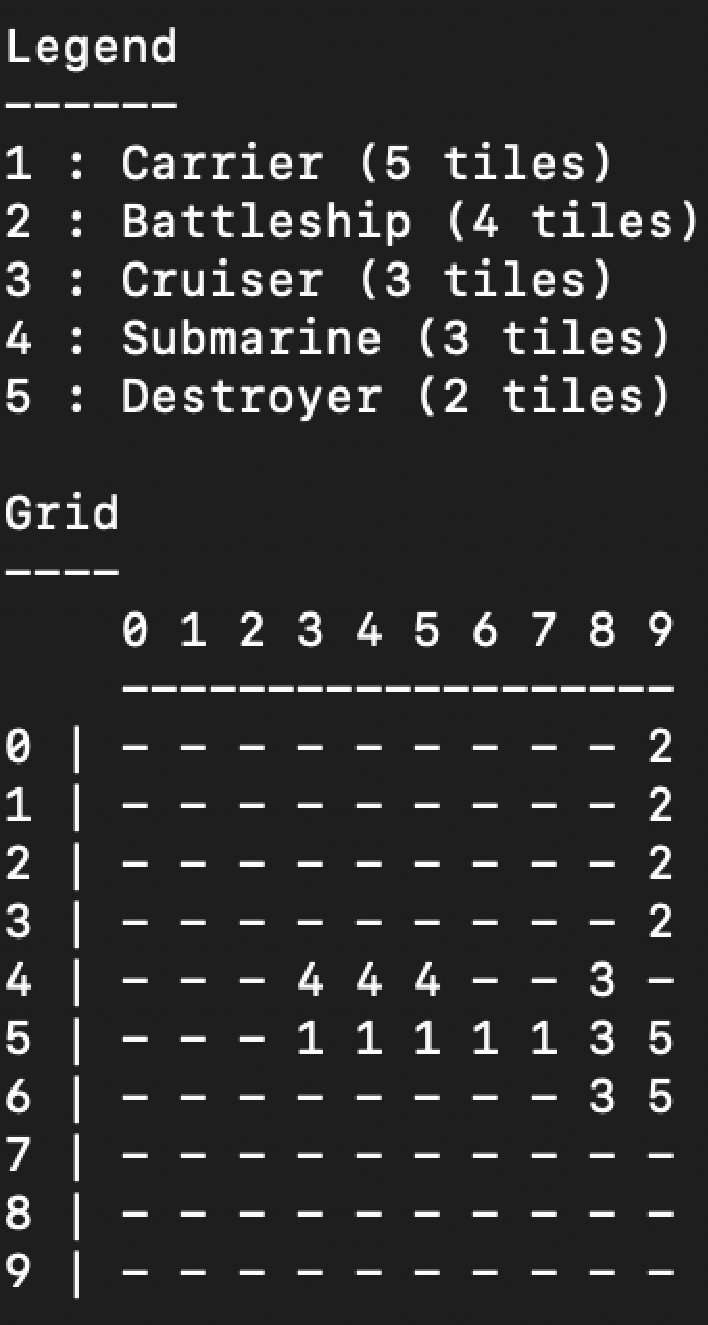
\includegraphics[scale=0.4]{resources/pdf/grid.pdf}
		\caption{Example of a game grid, with the conventions for coordinates.}
		\label{fig:grid}
	\end{figure}
	The grid deals mainly with placing the different ships and keeping their states up to date.
	\subsection{\texttt{ServerWorker}}
	This class is responsible for managing the server-side game. It is an extension of the \texttt{Thread} class. It is waiting for a request from the client :
	\begin{itemize}
		\item {\bf Request a new game} : when the client sends a request for a new game, the server instantiates the \texttt{GameManager} class and sends the client that the game has started;
		\item {\bf Request a shoot at a given position} : when the client sends a request to attack a position, the server reads the position, attacks this position using a \texttt{GameManager}'s method and sends back to the client the identifier of the affected ship (0 for no ship, greater than 0 for a ship) returned by the \texttt{GameManager};
		\item {\bf Request the game status} : when the client sends a request to obtain the status of the game, the server retrieves the list of position-ship pairs using a \texttt{GameManager} method. This list is converted to byte and sent to the client.
	\end{itemize}
	In all other cases where the client's request does not match one of the previous ones, a request error (\texttt{1 4}) is sent.
	\section{Multi-thread coordination}
	With each new connection on the server, the \texttt{BattleshipServer} class creates a new \texttt{Thread} (a new game, {\it i.e.} a new \texttt{GameManager}). When the game is over, the \texttt{Thread} dies (during a timeout or an exception, because the player can not send a request to indicate that it ends the game).\par
	In this case, no synchronization is required between threads. Indeed, each client plays its own part, so the threads do not share any object or segment of memory.
	\section{Limits}
	With the current protocol, it is not possible to know when the client has finished his game (if he wins, loses or prematurely leaves the game). So we have to catch an \texttt{IOException} to leave the current thread. It would be better to have a request dedicated to the one in the protocol so that the server can leave the game cleanly.\par
	In terms of robustness, checks are made in the client and in the server to verify properly that the requests are valid (or not). There are also local checks to prevent the client from entering a position that is not in the grid. An invalid request from the client is processed by the server, and vice versa. The client-server communication is thus a priori robust.\par
	However, the other classes of the game are not very robust : no verification of the validity of the parameters of the methods are performed. In theory, it is not possible that these parameters are false since all the client's inputs are checked and all the game data (size of the ships, grid size, ...) are implemented statically. It would be better, however, to implement custom exceptions in a more general context.
	\section{Possible improvements}
	Regarding the protocol, we could add other types of messages to have better communication between the client and the server. For example, a message that allows the client to indicate that they have finished a game so that the client stops the thread properly (or starts a new game).\par
	One could also have several error messages (instead of just having 1 4) to specifically tell the client what kind of error occurred.\par
	As part of this project, I made the choice of a very simple implementation so as not to clutter the code and keep only the essential.\par
	However, improvements could be made to make the game more {\it user-friendly} : the game grid could be displayed to the client (only with the positions he attacked) instead of just the positions in text and colors could also be used to represent ships on the grid. It could also be suggested to the client to restart a game when it finishes one (instead of simply stopping the execution of the client).\par
	In a more general context, a graphical interface could even be developed.
\end{document}
